\documentclass[a4paper,12pt]{book}
\usepackage[utf8]{inputenc}
\usepackage{pscyr}          % Нормальные шрифты
\usepackage[russian]{babel} %
\usepackage{graphicx}
\usepackage[left=2cm,right=2cm,top=2cm,bottom=2cm,bindingoffset=0cm]{geometry}
\usepackage{wrapfig}   % обтекаемые текстом блоки
\usepackage{soulutf8}  % выделение текста
\usepackage{xcolor}    % выделение цветом
\usepackage{array}
\usepackage{booktabs}
\usepackage{multirow,bigdelim}
\usepackage{hhline}
\usepackage{tabularx}
\usepackage{hyperref}
\usepackage{amsmath}
\usepackage{nccboxes}
\usepackage{mathtext}

\hypersetup{pdftitle={Электромагнитные переходные процессы}}  % метаданные PDF
\hypersetup{pdfauthor={Сергей Александрович Ульянов}}
\hypersetup{pdfcreator={LaTeX}}
\hypersetup{pdfproducer={https://github.com/wyfinger/Ulianov1970}}

\bibliographystyle{unsrt} % сортировка литературы в порядке упоминания (не как в книге)

%\hypersetup{ pdfborder={0 0 0}} % чтобы ссылки не выделялись

%\usepackage[dvips]{graphicx}
%\graphicspath{{pic/}}

\begin{document}

\author{Сергей Александрович Ульянов}
\title{Электромагнитные переходные процессы}
\
\date{1970}

\frontmatter
\maketitle
\tableofcontents

\mainmatter
\chapter{Основные сведения об электромагнитных переходных процессах}
\section{Основные определения}
Из всего многообразия электромагнитных переходных процессов в электрической системе наиболее распространенными являются процессы, вызванные:
\begin{enumerate} 
\item
включением и отключением двигателей и других приемников электроэнергии;
\item
коротким замыканием в системе, а также повторным включением и отключением (одновременным или 
каскадным) короткозамкнутой цепи;
\item
возникновением местной несимметрии в системе (например, отключение одной фазы линии передачи);
\item
несинхронным включением синхронных машин. 
\end{enumerate}

\so{Коротким замыканием} называют всякое не предусмотренное нормальными условиями работы замыкание между фазами, а в системах с заземленными нейтралями (или четырехпроводных)~---  также замыкание одной или нескольких фаз на землю (или на нулевой провод).

В системах с незаземленными нейтралями или с нейтралями, заземленными через специальные компенсирующие устройства, замыкание одной из фаз на землю называют \so{простым замыканием}. При этом виде повреждения прохождение тока обусловлено главным образом емкостью фаз относительно земли.

При возникновении короткого замыкания в электрической системе сопротивление цепи уменьшается (степень уменьшения зависит от положения точки короткого замыкания в системе), что приводит к увеличению токов в отдельных ветвях системы по сравнению с токами нормального режима. в свою очередь это вызывает снижение напряжений в системе, которое особенно велико вблизи места короткого замыкания.

Обычно в месте замыкания образуется некоторое переходное сопротивление, состоящее из сопротивления возникшей электрической дуги и сопротивлений прочих элементов пути тока от одной фазы к другой или от фазы на землю. Электрическая дуга возникает или с самого начала происшедшего повреждения как, например, при перекрытии или пробое изоляции, или через некоторое время, когда перегорит элемент, вызвавший замыкание. При замыканиях между фазами переходное сопротивление определяется главным образом сопротивлением электрической дуги.

\begin{wrapfigure}[10]{r}{0.4\linewidth} 
	\centering
%	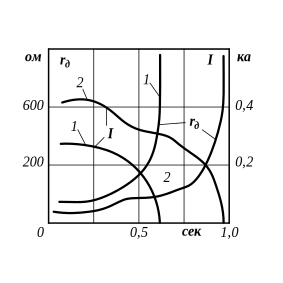
\includegraphics[width=0.5\linewidth]{1-1}
	\caption{}
	\label{fig:q}
\end{wrapfigure}

\begin{figure}
\centering
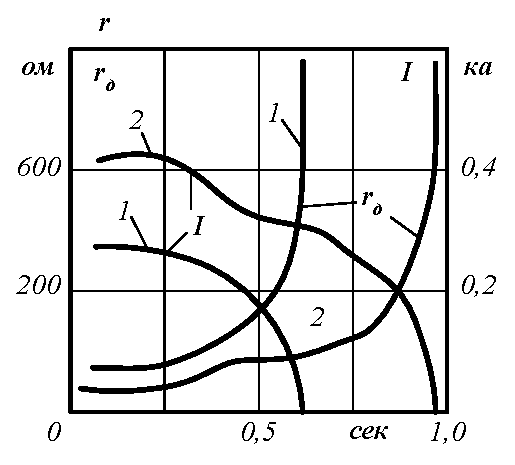
\includegraphics[width=0.7\linewidth]{a}
\caption{}
\label{fig:a}
\end{figure}


Когда токи достаточно велики (сотни ампер и более), сопротивление дуги приблизительно постоянно и по
своему характеру почти чисто активное. С уменьшением, тока и увеличением длины дуги, что имеет место в течение переходного процесса, ее сопротивление возрастает. Наглядной иллюстрацией такого изменения могут служить графики (рис. 1-1), полученные экспериментально при возникновении самопогасающих дуг на линиях
110~\textit{кв} с деревянными опорами.







\chapter{Общие указания к выполнению расчетов}

\section{Основные допущения}

Как отмечалось выше, расчет электромагнитного переходного процесса в современной электрической системе с учетом всех имеющих место условий и факторов чрезвычайно сложен и практически невыполним. Поэтому, чтобы упростить задачу и сделать ее решение практически возможным, вводят ряд допущений. Последние зависят прежде всего от характера и постановки самой задачи. Те допущения, которые вполне пригодны при решении одной задачи, могут быть совершенно неприемлемыми при решении другой.

Каждый из практических методов расчета, электромагнитных переходных процессов, в частности процесса при коротком замыкании, основан на некоторых допущениях, касающихся преимущественно возможности использование упрощённых представлений об изменении свободных токов в сложных схемах с несколькими источниками, о разных способах учета автоматического регулирования возбуждения синхронных машин и т.~п. C ними читатель познакомится в ходе дальнейшего изложения материала. Здесь же остановимся только на тех основных допущениях, которые обычно принимают при решении большинства практических задач, связанных с определением токов и напряжений при электромагнитных переходных процессах. К  числу таких допущений следует отнести:

\begin{enumerate} 
	\item
	отсутствие насыщения магнитных систем. При этом все схемы оказываются линейными, расчет которых значительно проще; в частности, здесь могут быть использованны любые формы принципа наложения.
	\item
	Пренебрежение токами намагничивания трансформаторов и автотрансформаторов. Единственным исключением их этого допущения является случай, когда трехстержневой трансформатор с соединением обмоток $ Y_{0}/Y_{0} $ включен на напряжение нулевой последовательности (см.~\colorbox{red}{§12-5}).
	\item
	Сохранение симметрии трехфазное системы. Оня нарушается обычно лишь для какого-либо одного элемента, что происходит в результату его повреждения, или преднамеренно по специальным соображениям (см. гл.~\colorbox{red}{15}).
	\item
	Пренебрежение емкостными проводимостями. Это допущение обычно является, уместным и заметно не искажает результаты решения, если в рассматриваемой схеме нет продольной компенсации индуктивности цепи, а также дальних линий передач напряжением выше 220~\textit{кв}. При рассмотрении простых замыканий на землю (см.~§\colorbox{red}{17-2}) это допущение, разумеется, совсем непригодно, так как в данном случае ток замыкается именно через емкостные проводимости.
	\item
	Приближенный учет нагрузок. В зависимости от стадии переходного процесса нагрузку приближенно характеризуют некоторым постоянным сопротивлением, обычно чисто индуктивным (см.~\colorbox{red}{§5-4 и §6-5}).
	\item
	Отсутствие активных сопротивлений. Это допущение в известной мере условно. Оно приемлемо при определении начальных и конечных значений отдельных величин, характеризующих переходный процесс в основных звеньях высокого напряжения электрической системы; при этом приближенный учет активных сопротивлений находит отражение при оценке постоянных времени затухания свободных составляющих рассматриваемых величин. В тех же случаях, когда подобный расчет проводится для протяженной кабельной или воздушной сети с относительно небольшими сечениями проводников (особенно линии со стальными проводами), а также для для установок и сетей напряжением до 1~\textit{кв}, данное допущение непригодно (см.~\colorbox{red}{гл. 17}).
	\item
	Отсутствие качаний синхронных машин. Если задача ограничена рассмотрением лишь начальной стадии переходного процесса (т.~е. в пределах 0,1--0,2~\textit{сек} с момента нарушения режима до отключения повреждения), это допущение обычно не вносит заметной погрешности (особенно в токе в месте повреждения). Однако при возникновении существенных качаний или выпадении машин из синхронизма достаточно надежный результат может быть получен лишь с учетом (хотя бы приближенным) такого процесса (см.~\colorbox{red}{гл. 19}).
\end{enumerate}

\section{Понятие о расчетных условиях}

В соответствии с целевым назначением проводимого на практике расчета электромагнитного переходного процесса устанавливают исходные расчетные условия. Они весьма разнообразны и при решении разных задач могут быть даже противоположными.

Так, например, для выбора выключателя по условиям его работы при коротком замыкании должны быть определены соответствующие возможные наибольшие величины тока короткого замыкания. С этой целью исходят из предположения, что короткое замыкание происходит в то время, когда включено наибольшее число генераторов, что вид короткого замыкания такой, при котором ток достигает наибольшей величины, что короткое замыкание металлическое и что оно произошло непосредственно у выводов самого выключателя. Помимо того, здесь устанавливают расчетное время размыкания контактов выключателя и цикл производимых им операций (включение и отключение).

Для выбора трубчатого разрядника требуется знать не только наибольшую, но и возможную наименьшую величину тока короткого замыкания, для определения которой, разумеется, должны быть приняты совсем иные расчетные условия.

Большое разнообразие расчетных условий встречается при выполнении расчетов для выбора и настройки устройств релейной защиты и автоматики. В них устанавливаются исходные предшествующие режимы заданной системы, число и расположение заземленных нейтралей, виды повреждений, и последовательность отключения поврежденного участка и т.~п.

При решении вопроса гашения поля синхронной машины в качестве расчетного режима может быть как режим короткого замыкания, так и холостого хода.

Приведенные примеры показывают, сколь велико разнообразие расчетных условий. Обоснование расчетных условий для конкретных технических задач (с учетом вероятности отдельных факторов) является одним из важных вопросов соответствующих специальных дисциплин.

\section{Система относительных единиц}

Представление любых физических величин не в обычных для них соответствующих именованных единицах, а в относительных, безразмерных единицах позволяет существенно упростить некоторые теоретические выкладки и придать им более общий характер. Равным образом и в практических расчетах такое представление величин придает результатам большую наглядность и позволяет быстрее ориентироваться в порядке определяемых значений. Благодаря этому система относительных единиц широко используется, хотя на первый взгляд она может казаться несколько искусственной и даже излишней.

С выражением величин в относительных единицах (в долях или процентах) читатель уже встречался при изучении электрических машин, где реактивности обычно выражают в долях единицы, напряжения короткого замыкания трансформаторов --- в процентах, пусковые токи и моменты асинхронных двигателей --- в кратностях от их номинальных значений и т.~д. Теперь нам нужно познакомиться с системой относительных единиц в более широком аспекте, имея в виду использование ее при решении различных вопросов и задач для схем с произвольным числом всевозможных элементов.

Напомним, что под относительным значением какой-либо величины следует понимать ее отношение к другой одноименной величине, выбранной за единицу измерения. Следовательно, чтобы выразить отдельные величины в относительных единицах, нужно прежде всего выбрать те величины, которые должны служить соответственными единицами измерения, или, как говорят, установить базисные единицы (или условия).

Пусть за базисный ток и базисное междуфазное напряжение приняты некоторые произвольные величины $ I_{\mbox{б}} $ и $ U_{\mbox{б}} $. Тогда базисная мощность трехфазной системы, очевидно, будет:

\begin{equation}
	\label{eq:chap2 S_baz}
	S_{\mbox{б}} = \sqrt{3}U_{\mbox{б}}I_{\mbox{б}}
\end{equation}

и базисное сопротивление

\begin{equation}
	\label{eq:chap2 z_baz}
	z_{\mbox{б}} = \frac{U_{\mbox{б}}}{\sqrt{3}I_{\mbox{б}}}
\end{equation}

т.~е. оно подчинено закону Ома, чтобы обеспечить тождественную запись этого закона как в именованных, так и в относительных единицах.

Как видно, из четырех базисных единиц $ I_{\mbox{б}} $, $ U_{\mbox{б}} $, $ S_{\mbox{б}} $ и $ z_{\mbox{б}} $ только две могут быть выбраны произвольно, а две другие уже получаются из указанных соотношений. Фазные и междуфазные базисные напряжения, а также фазные и линейные базисные токи связаны между собой известными соотношениями для симметричной трехфазной системы. Следует особо подчеркнуть, что выбранные базисные единицы служат для, измерения как полных величин, так и их составляющих (активных, реактивных и~пр.).

Таким образом, при выбранных базисных условиях относительные значения э.~д.~с., напряжения, тока, мощности и сопротивления будут:

\begin{equation}
	\label{eq:E_baz_otn}
	\underset{*}{E_{\mbox{б}}} = \frac{E}{U_{\mbox{б}}}
\end{equation}











\backmatter
% bibliography, glossary and index would go here.

\end{document}